% LaTex file for Stephen Balakirsky's RITA 2014 submission
%
\documentclass{llncs}
%
\usepackage{makeidx}  % allows for indexgeneration
%
% my additional packages
\usepackage{graphicx}
\usepackage{multirow,array}
\usepackage{rotating} % for sideways
\usepackage{amsmath}
\usepackage{amsthm}
%\usepackage{algorithm2e}
\usepackage[linesnumbered, boxed, figure]{algorithm2e}
%
% zeid's definitions
\newcommand{\class}[1] {\textit{#1}}
\newcommand{\const}[1] {$\mathit{#1}$}
\newcommand{\objvar}[1] {$\mathsf{#1}$}
\newcommand{\stvar}[1] {\textsf{#1}}
%
%
\begin{document}
%
\frontmatter          % for the preliminaries
%
\pagestyle{headings}  % switches on printing of running heads
\addtocmark{Hamiltonian Mechanics} % additional mark in the TOC
%
%
\mainmatter              % start of the contributions
%
\title{An Ontology Based Approach to Action Verification for Agile Manufacturing}
%
\titlerunning{Agile Manufacturing}  % abbreviated title (for running head)
%                                     also used for the TOC unless
%                                     \toctitle is used
%
\author{Stephen Balakirsky\inst{1} \and Zeid Kootbally\inst{2}}
%
\authorrunning{Stephen Balakirsky et al.} % abbreviated author list (for running head)
%
%%%% list of authors for the TOC (use if author list has to be modified)
\tocauthor{Stephen Balakirsky, Zeid Kootbally}
%
\institute{Georgia Tech Research Institute, Atlanta, GA 30332, USA,\\
\email{stephen.balakirsky@gtri.gatech.edu},\\ WWW home page:
\texttt{unmannedsystems.gtri.gatech.edu}
\and
University of Maryland, College Park, MD zip, USA,\\
\email{zeid.kootbally@umd.edu},\\ WWW home page:
\texttt{www.washingtonpost.com}
}

\maketitle              % typeset the title of the contribution

\begin{abstract}
The abstract should summarize the contents of the paper
using at least 70 and at most 150 words. It will be set in 9-point
font size and be inset 1.0 cm from the right and left margins.
There will be two blank lines before and after the Abstract. \dots
\keywords{manufacturing, ontology, robotics}
\end{abstract}
%
%
\section{Introduction}
A failure is any change, design, or manufacturing error that renders a component, assembly, or system incapable of performing its intended function \cite{Collins93}. In kitting, failures can occur for multiple reasons including: equipment not being set up properly, tools and/or fixtures not being properly prepared, and improper equipment maintenance. Part/component availability failures can be triggered by inaccurate information on the location of the part, part damage, incorrect part types, or part shortage due to delays in internal logistics. In order to prevent or minimize failures, a disciplined approach needs to be implemented to identify the different ways a process design can fail before impacting the productivity.

Even though today's state-of-the-art industrial robots are capable of sub-millimeter accuracy \cite{RobotAccuracy}, they often lack the sensing
necessary to detect failures and the programming required to cope with and correct the failure. This is due to the fact that they are often programmed
by an operator using crude positional controls from a teach pendent. These teach pendent programs are highly repeatable, which provides 
utility for large-batch, error-free operation. However, the cyclic program that repeats identical operations does not lend itself well to adaptation for 
error failure mitigation. In fact, producing a program to correct a perceived failure would require that the cell be taken off-line
for additional human-led teach pendent programming. In addition, 
most cells lack the ability to sense that an failure occurred and  lack programming (that would have had to be teach pendent entered) to cope
with error conditions, thus making it impossible for the cell to recover from errors.
This leads to faulty products being sent down the line, and/or downtime for the cell as errors are detected and corrected.

For small batch processors or other customers who must frequently change their line configuration or desire to perform complex operations
with their robots, this frequent downtime and lack of error correction/detection may be unacceptable. The robotic systems of tomorrow need to be capable, flexible, and agile.  
These systems need to perform their duties at least  as well as human counterparts, be quickly re-tasked to other operations, cope with a wide 
variety of unexpected environmental and operational changes, and be able to detect and correct errors in operation. 
To be successful, these systems need to combine domain expertise, knowledge of their own skills and limitations, and both semantic and geometric 
environmental information.

The IEEE Robotics and Automation Society's Ontologies for Robotics and Automation Working group has taken the first steps in creating the 
infrastructure necessary for such a system, while the Industrial Subgroup has applied this infrastructure to create a sample kit building
system.  This work is presented in Balakirsky et al. \cite{balakirsky2013} which describes the construction of a robotic kit building
system that is able to cope with environmental and task changes without operator intervention. This article extends that work to utilize
the same infrastructure to allow for the detection and correction of action errors in the system.

The organization of the remainder of this paper is as follows. Section \ref{sect:kitting} describes the domain of kit building. Section \ref{sect:overview} presents
an overview of the software system architecture for the robot cell. Section \ref{sect:operation} presents results of this work, and Section \ref{sect:future} presents
conclusions and future work.
%
%
\section{Kitting}
\label{sect:kitting}
Today's advanced manufacturing plants utilize mixed-model assembly where multiple product variants are built on the same line.  
According to Jim Tetreault, Ford’s vice president of North America Manufacturing, 
new Ford assembly facilities are able to build a full spectrum of vehicles on the same assembly line \cite{James2011}. One of the technologies that makes this possible
is the use of assembly kits.  Bozer and McGinnis \cite{Bozer1992} describe a kit as ``a specific
collection of components and/or subassemblies that together (i.e., in the same container) support one or more assembly
operations for a given product or shop order''. These  kits provide a synchronous material flow, where parts and components move to 
assembly stations in a just-in-time manner. The kits provide workers with the parts and tools that they need (which may vary from 
vehicle model to vehicle model) in the sequence that they need them. The use of kitting also allows a single delivery system to feed
multiple assembly stations thus saving manufacturing or assembly space \cite{Medbo2003} and provides an additional inspection opportunity 
that allows for the detection of part defects before they impact assembly operations. The individual operations of the station 
that builds the kits may be viewed as a specialization of the general
bin-picking problem \cite{Schyja2012} where parts are picked from one or more part bins or trays and placed into specific slots in a kit tray.

For our sample implementation, we assume that the robot cell is building one of several possible kit configurations. At execution time, the
cell has a set kit to build, but does not know the precise location of the kit tray, the part trays, or the location of individual parts in the part tray.
When a human builds a kit, they are able to inspect each part before adding it to the kit tray. This provides an additional level of quality control and
is an aspect that is desirable to have in our robotic system. During kit construction,
a robot performs a series of pick-and-place operations
in order to construct the kit. These operations include:
\begin{enumerate}
\item Pick up an empty kit and place it on the work table.
\item Pick up multiple component parts, inspect them, and place them in the kit.
\item Pick up the completed kit and place it in the full kit storage area.
\end{enumerate}
Each of these may be a compound action that includes
other actions such as end-of-arm tool changes, path planning,
and obstacle avoidance. The items that are being placed in the kit may be of varying size and shape and have various grasping and inspection
requirements.
%
\begin{figure}[htb!]
\begin{center}
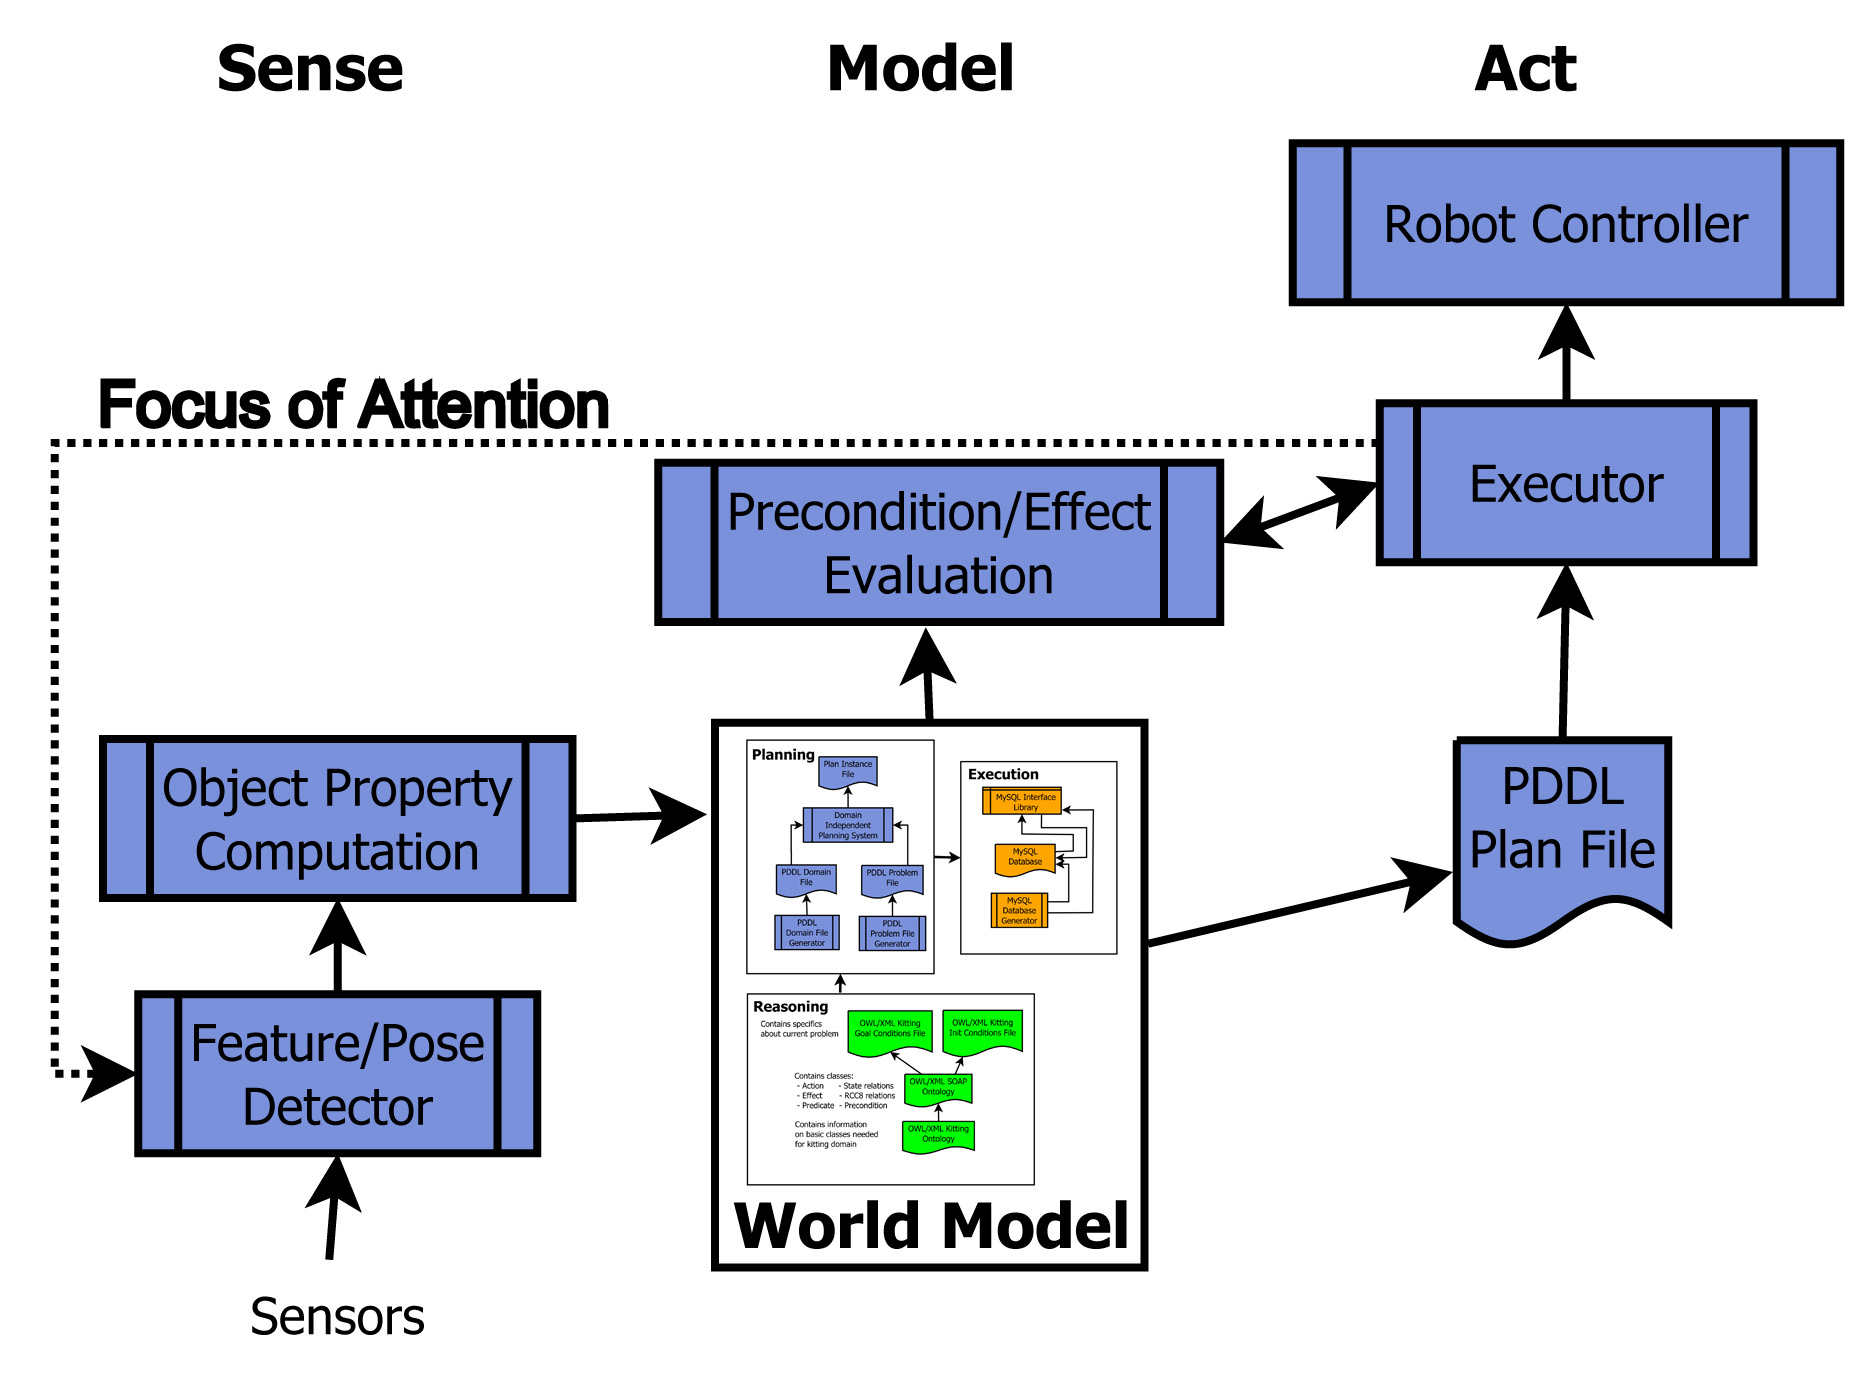
\includegraphics[width=8.5cm]{images/RITAExecution.jpg}
\caption{Major components that make up the Sense--Model--Act paradigm of the kitting station.}
\label{fig:SenseModelAct}
\end{center}
\end{figure}
%
%
\section{System Overview}
\label{sect:overview}
The kitting system that has been implemented as part of this work is a deliberative intelligent system based on the 4D/RCS 
reference model architecture\cite{Albus2000}. This architecture is a hierarchical architecture in which each echelon or level
follows a sense-model-act paradigm. The basic structure of the system may be seen in Figure \ref{fig:SenseModelAct}.
%
\subsection{Sense}
\label{subsection:Sense}
In order to sense action failures associated with kit building, it is necessary to be able to detect the six-degree of freedom pose of relevant objects in the
world. One issue with pose detection is the large number of potential target objects and object classes in the world. 
Both the number of objects and potential classes can be reduced by intelligently
selecting critical objects of interest that are tagged with predicted locations and object class for the sensor system to track. This object selection, 
also known as focus of attention, is guided by
the executor process with knowledge obtained from preconditions and effects of planned actions.
Actual algorithm development for pose and object detection is an active research area, and is beyond the scope of this article. 

For our purposes, 
we have assumed the use of a high-quality
system that is capable of recognizing a limited variety of items in a controlled environment and then determining the item's pose. This is accomplished through
simulation by using the Unified System for Automation and Robot Simulation (USARSim) \cite{Balakirsky2007}. As described in Section \ref{sect:future}, 
we intend to relax this assumption in the near future.
%
\begin{figure}[htb!]
\begin{center}
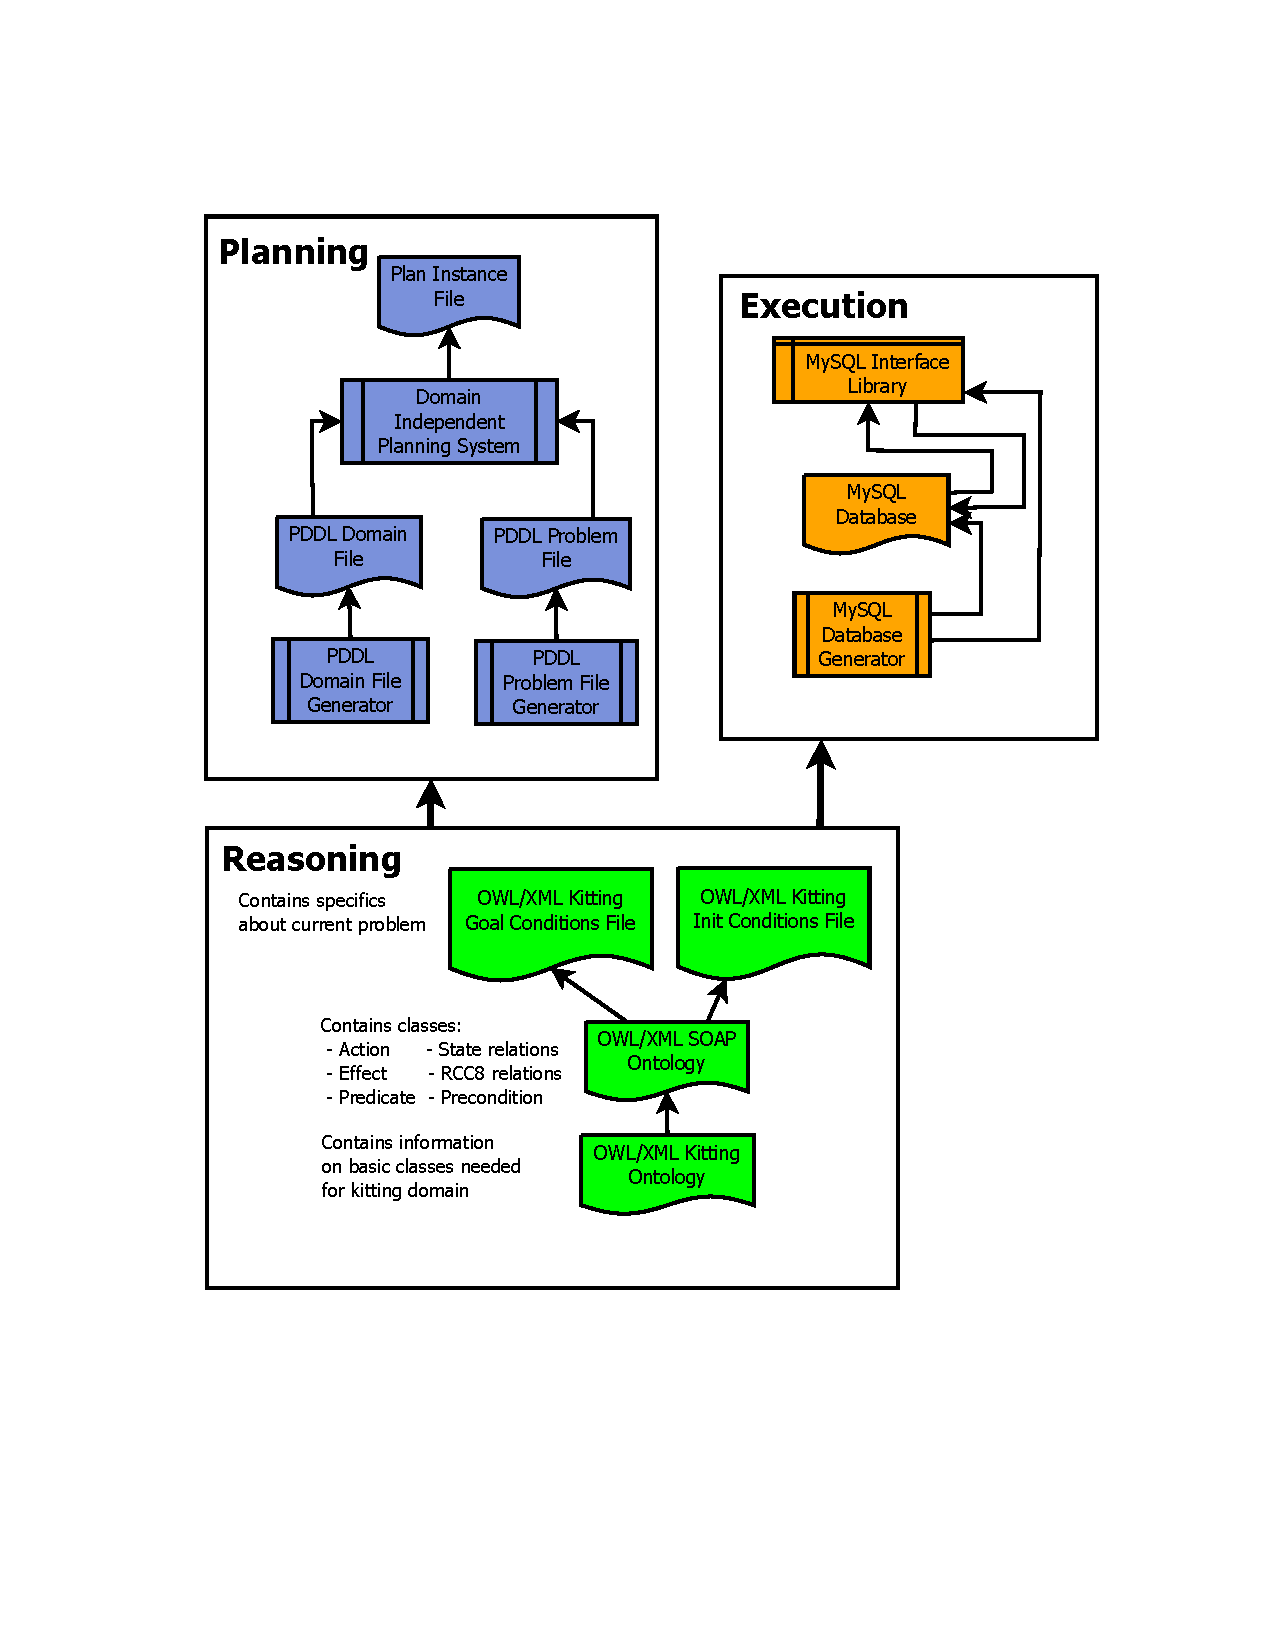
\includegraphics[width=8.5cm]{images/RITAWorldModel.pdf}
\caption{System World Model - The world model contains an ontology shown in green,
a Planning Domain Definition Language (PDDL) specification shown in blue, and a dynamic database shown in orange.}
\label{fig:WorldModel}
\end{center}
\end{figure}
%
\subsection{Model}
\label{subsection:Model}
The world model that is being utilized is shown in Figure \ref{fig:WorldModel}. The model contains knowledge that is structured specifically for
reasoning, planning, and execution. All of the concepts necessary for the manufacturing domain under test are
encoded in the ontology that resides in the reasoning section of the model. The planning and execution sections of the model are automatically generated from
this section.
\subsubsection{Ontology --}
\label{sect:Ontology}
The reasoning portion of the world model is designed to contain all of the information needed to reason over and solve complex manufacturing
problems. The knowledge is represented in an ontology that is structured in three levels. The first part of the ontology is an upper ontology
that contains generic information and classes that are needed for the domain of kit building. 

This area of the ontology contains information on basic elements such as a ``point" which is defined as a class that contains a name 
and a three-dimensional quantity, as well as complex types such as a ``part'', which is
shown in Figure \ref{fig:part}, and
contains elements such as a the part's shape, stock keeping unit (SKU) number, and location. This information is utilized to create parameters for the Planning World
Model and the skeleton tables for the mySQL database of the Execution World Model.
%
\begin{figure}[htb!]
\begin{center}
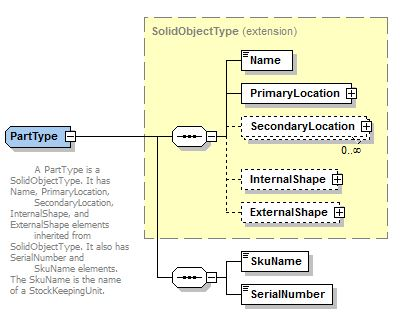
\includegraphics[width=8.5cm]{images/Part.jpg}
\caption{Description of the PartType class that is designed to contain both static and dynamic information about particular parts.}
\label{fig:part}
\end{center}
\end{figure}
%
Both static and dynamic information is represented in this
ontology and is automatically transitioned into the Planning and Execution areas of the world model. During system
operation,  dynamic information is updated in the Execution World Model.
More information on this portion of the ontology may be found in \cite{Balakirsky2012-1}.


The second level of the ontology (known as States, Ordering constraints, Actions, and Predicates or SOAP) contains the high-level concept of an action and all of the concepts 
that are required to support an action. In this case, a Planning Domain Definition Language (PDDL) \cite{PDDL} action is being represented, and this action is defined
 as an operator that causes one or more properties of an 
instance to change. Before this action may be
performed, certain preconditions must be satisfied, and after the action is performed, certain effects will take place. The action accepts parameters that specify the particular
instances that will be affected, where an instance refers to a physical object in the world. The classes used to represent the actions in the ontology are provided in the
enumerated list shown below. The naming convention utilized follows the OWL \cite{OWLoverview} implementation of the ontology.

ZEID, FIX HERE!

\begin{enumerate}
\item \class{Action} -- An \class{Action} has a \class{Precondition} and an \class{Effect}. An \class{Action} has a \class{ParameterList} that contains all the parameters for an action. An action has unique name.
\item \class{ParameterList} -- Actions may have multiple parameters of different types. Each one of these types is represented by a class in the upper ontology. The \class{ParameterList} has \class{Parameter}s that are instances from the upper ontology. The order of the parameters in an  action also needs to be represented in the ontology. OWL has no built-in structure to represent an ordered list, instead, the \class{Parameter}, uses \emph{hasParameter\_Next} to point to the next parameter in \class{ParameterList}.
\item \class{Precondition} -- A \class{Precondition} can consist of a \class{Predicate}, a \class{Function}, a \class{FunctionBool}, or a combination of these three classes. A \class{Precondition} belongs to one \class{Action}.
\item \class{Effect} -- An \class{Effect} can consist of a \class{Predicate}, a \class{Function}, \class{FunctionBool}, or a combination of these three classes. An \class{Effect} belongs to one \class{Action}. A negative \class{Predicate} is represented with the declaration of \emph{hasEffect\_Predicate} within the OWL built-in property assertion \texttt{owl:NegativePropertyAssertion}.
\item \class{Predicate} -- A \class{Predicate} has a unique name  of type \texttt{string}. A \class{Predicate} has a reference parameter and a target parameter. A reference parameter is the first parameter in the \class{Predicate}'s list and the target parameter is the second parameter in the parameter's list. A \class{Predicate} cannot have more than two parameters due to the inherent definition of \class{Predicates}. In the case where a \class{Predicate} has only one parameter, it is assigned to the reference parameter. Reference and target parameters are one of the parameters defined for the \class{Action} to which the \class{Predicate} belongs.
    
    The meaning of reference and target parameters lies in the definition of a state variable. We recall the following definition of a state variable $\mathrm{x: A_1\times \dots\times A_i\times S\rightarrow B_1\cup\dots\cup B_j}$ ($i, j\geq 1$) that is used to convert state variables into predicates as follows:

\begin{itemize}
 \item $\mathrm{A_1\times \dots\times A_i\times S\rightarrow B_1\cup\dots\cup B_j}$ ($i, j\geq 1$)
  \begin{itemize}
  \item \stvar{predicate\_1}($\mathcal{A,B}$)
  \item \ldots
  \item \stvar{predicate\_n}($\mathcal{A,B}$)
  \end{itemize}
\end{itemize}

Where $\mathcal{A} \in \mathrm{\{A_1,\ldots,A_i\}}$ and $\mathcal{B} \in \mathrm{\{B_1,\ldots,B_i\}}$ ($i, j\geq 1$)

From this methodology, we have defined a predicate's parameter as a reference parameter if the parameter belongs to the set $\mathcal{A}$. Similarly, we have defined a predicate's parameter as a target parameter if the parameter belongs to the set $\mathcal{B}$. For instance, the predicate \texttt{(part-location-robot ?part ?robot)} has \texttt{?part} as the reference parameter and \texttt{?robot} as the target parameter. This convention has been used in our ontology to define these two distinct types of parameters.

\item \class{Function} -- A \class{Function} has a unique name  of type \texttt{string}. A \class{Function} has a reference parameter and a target parameter. The same rules apply to the definition and use of these two types of parameters as the ones defined for \class{Predicate}.
\item \class{FunctionBool} -- \class{FunctionBool} has one or more subclasses that represent the type of relation between two \class{Functions}. For example, the relation depicted at line 13--14 in is represented in the subclass \class{IntLesserThanInt}. Subclasses of \class{FunctionBool} have a first \class{Function} that represents the \class{Function} on the left side of the operator. Subclasses of \class{FunctionBool} have a second \class{Function} that represents the \class{Function} on the right side of the operator.
\end{enumerate}

The third level of the ontology contains specific instances needed for a particular kitting domain. For example, it will contain the definition of the finished kits that may be
constructed and specific information on the individual parts. One of the goals of this framework is to introduce additional agility into the kit building process. Therefore,
partial information is accepted and even encouraged for this area of the ontology. For the example of a part shown in Figure \ref{fig:part}, information on the SKU, grasp points 
(part of the ExternalShape or InternalShape), and name would be expected to be available at runtime. Information on the location of the part (PrimaryLocation) may not
become valid until after a sensor processing system has identified and located the particular part.

\subsubsection{Planning --}
The Planning Domain Definition Language (PDDL)  is an attempt by the domain independent planning community to formulate a standard language for planning. A community of planning researchers has been producing planning systems that comply with this formalism since the first International Planning Competition held in 1998. This competition series
continues today, with the seventh competition being held in 2011. PDDL is constantly adding extensions to the base language in order to represent more expressive problem domains. The representation in the world model is based on PDDL Version 3.

By placing the knowledge in a PDDL representation, the use of an entire family of open source planning systems such as the forward-chaining partial-order planning system from Coles et al. \cite{Coles.ICAPS.2010}
is enabled. In order to operate, the PDDL planners require a PDDL file-set that consists of two files that specify the domain and the problem.
From these files, the planning system creates an additional static plan file.

This plan file contains a sequence of actions that will transition the system from the initial state to the goal state. In order to maintain flexibility, it is desired that detailed information that is subject to change should be ``late-bound'' to the plan. In other words, specific information is acquired directly before that information needs to be used by the system. This allows for last minute changes in this information. For example, the location of a kit tray on a work table may be different from run to run. However, one would like to be able to use the same planning sequence for constructing the kit independent of the tray's exact position.
To compensate for this lack of exact knowledge, the plans that are generated by the PDDL planning system contain only high-level actions.

As seen in Figure \ref{fig:WorldModel}, the planning world model framework contains generators that read the ontology and create
a standard PDDL domain and PDDL problem file. Any of the family of PDDL Version 3 compatible planning systems is then able to be
run on these files to create the static plan instance file. A representation of this plan may be stored in the ontology for future use.

\subsubsection{Execution --}
The execution world model is also built automatically from the ontology. This world model consists of a mySQL database and C++ and Java
interfaces that provide for easy access to the data. The table skeletons are generated from the kitting ontology, and the tables are initially populated
with information from the initial and goal condition files. During plan execution, the executor guides the sensor processing system
in updating the information in 
this section of the world model. All of the data structures encoded in the ontology are included in this representation. 
%An example 
%of the data tables that are created may be seen in Figure ?? for the Part class that is shown in Figure \ref{fig:part}. 
%
\subsection{Act}
\label{subsection:Act}
The actions that take place in the kitting work cell are coordinated by the Executor as illustrated in Figure \ref{fig:SenseModelAct}.  The Executor
reads PDDL actions as input and outputs a standardized set of low-level robot commands developed at the National Institute of Standards
and Technology known as the  Canonical Robotic Command Language \cite{Balakirsky2012-1}. 

Before and after each high-level command
is executed, the Executor sends focus of attention information into the sensor processing system. This allows the sensor processing system to compute
the appropriate predicate relations that are required to verify the conditions necessary to carry out an action and that an action's execution has
been successful. Information on predicates is written to the world model by the sensing system and read from the world model by the executor.
%
\\
\begin{algorithm}[h!]

 \KwData{ $kitToBuild$ }
 \KwResult{reports success or failure}
 	retrieve instance $PDDLInstance$ to construct kit $kitToBuild$\;
 	\For{each action $\textbf{A}$ in $PDDLInstance$}{
 		\For{each precondition $\textbf{P}$ of action $\textbf{A}$} {
			\If{$PredicateEvaluation(P)=false$}{
				report failure\;
			}
 		}
 		create set $S$ of Canonical Robot Language Commands\;
 		send set $S$ to Robot Controller for execution\;
 		\For{each effect $\textbf{E}$ of action $\textbf{A}$} {
			\If{$PredicateEvaluation(E)==false$}{
				report failure\;
			}
 		}
 		report action success\;
 	}
 	report plan success\;
\caption{{\sc BuildKit} -- Sequences the actions necessary to build a kit.}
\label{fig:buildkit}
\end{algorithm}
%
\section{System Operation}
\label{sect:operation}
In order to construct a kit, the kitting system steps through each action in
the precomputed PDDL plan. Failures are searched for both before and after execution of 
each action. The overall process, known as {\sc BuildKit} is shown in Figure
\ref{fig:buildkit}. 

This process begins by retrieving a planning instance that has been 
precomputed to solve the construction of the requested kit (Line 1 of 
Figure \ref{fig:buildkit}). This is a high-level PDDL
plan that is not grounded to actual parts or locations. It contains information
on the named storage location for classes of parts (individual SKU numbers), 
the quantity of each SKU that is required by the kit, and a build order (a sequence
of SKUs to be added to the kit). Additional information on the appropriate
end-of-arm tooling required to grip each part is also included.

This planning instance is decomposed into individual actions that must
be successfully carried out to complete the construction of the kit (the
{\it for} loop beginning at line 2 of Figure \ref{fig:buildkit}). At this point,
preconditions of the action are examined to assure that the action to be attempted
is valid. If any of the action's preconditions are not able to be validated,
a failure is reported; otherwise, the action is approved for execution.

\subsection{Predicate Validation}
The procedure for validating predicates is shown in Figure \ref{fig:predicateEval}. In line 1 of this algorithm, the world
model is queried for the pose and class of each relevant 
parameter of the predicate. The information returned is the 
latest knowledge that has been recorded by the sensor processing
system and is not guaranteed to be up-to-date. This predicted
knowledge is sent as a focus of attention indicator to the sensor
processing system, and the sensor processing system is instructed to
update the predictions in the world model with current observations.
While the location of objects is the basis for predicate evaluation,
it is not sufficient to determine a predicates truth value. The
concept of ``Spatial Relations'' is used as an aid to compute the
final truth values.

\subsubsection{Representation of Predicates with State Relations --}
There are three types of spatial relations that are each represented as a separate class in the ontology. Each class is described below.
\begin{itemize}
 \item \class{RCC8\_Relation}: RCC8 \cite{Wolter2000} is a well-known and cited approach for representing the relationship between two regions in Euclidean space or in a topological space. Based on the definition of RCC8, the class \class{RCC8\_Relation} consists of eight possible relations, including Tangential Proper Part (TPP), Non-Tangential Proper Part(NTPP), Disconnected (DC), Tangential Proper Part Inverse (TPPi), Non-Tangential Proper Part Inverse (NTPPi), Externally Connected (EC), Equal (EQ), and Partially Overlapping (PO). In order to represent these relations in all three dimensions for the kitting domain, we have extended RCC8 to a three-dimensions space by applying it along all three planes (x-y, x-z, y-z) and by including cardinal direction relations ``+'' and ``-''. In the ontology, RCC8 relations and cardinal direction relations are represented as subclasses of the class \class{RCC8\_Relation}. Examples of such classes are \class{X-DC}, \class{X-EC}, \class{X-Minus}, and \class{X-Plus}.

 \item \class{Intermediate\_State\_Relation}: These are intermediate level state relations that can be inferred from the combination of RCC8 and cardinal direction relations. For  instance, the intermediate state relation \textbf{Contained-In} is used to describe object \textit{obj1} completely inside object \textit{obj2} and is represented with the following combination of RCC8 relations:
\begin{gather}
\textbf{Contained-In}(\textit{obj1}, \textit{obj2}) \rightarrow   \notag\\
(\texttt{x-TPP}(\textit{obj1}, \textit{obj2}) \vee \texttt{x-NTPP}(\textit{obj1}, \textit{obj2})) \wedge \notag\\
(\texttt{y-TPP}(\textit{obj1}, \textit{obj2}) \vee \texttt{y-NTPP}(\textit{obj1}, \textit{obj2})) \wedge \notag\\
(\texttt{z-TPP}(\textit{obj1}, \textit{obj2}) \vee \texttt{z-NTPP}(\textit{obj1}, \textit{obj2}))\notag
\end{gather}
In the ontology, intermediate state relations are represented with the OWL built-in property \texttt{owl:equivalentClass} that links the description of the class \class{Intermediate\_State\_Relation} to a logical expression based on RCC8 relations from the class \class{RCC8\_Relation}.
 \item \class{Predicate}: The representation of predicates has been illustrated in Section. In this section we discuss how the class \class{Predicate} has been extended to include the concept of ``Spatial Relation''. The truth-value of predicates can be determined through the logical combination of intermediate state relations. The predicate \class{kit-location-lbwk}(\textit{kit}, \textit{lbwk}) is true if and only if the location of the kit \textit{kit} is in the large box with kits \textit{lbwk}. This predicate can be described using the following combination of intermediate state relations:
\begin{gather}
\textsf{kit-location-lbwk}(\textit{kit}, \textit{lbwk}) \rightarrow   \notag\\
\textbf{In-Contact-With}(\textit{kit}, \textit{lbwk}) \wedge \notag\\
\textbf{Contained-In}(\textit{kit}, \textit{lbwk}) \notag
\end{gather}
As with state relations, the truth-value of predicates is captured in the ontology using the \texttt{owl:equivalentClass} property that links the description of the class \class{Predicate} to the logical combination of intermediate state relations from the class \class{Intermediate\_State\_Relation}.

As seen in Section \ref{sect:Ontology}, a predicate can have a maximum of two parameters. In the case where a predicate has two parameters, the parameters are passed to the intermediate state relations defined for the predicate, and are in turn passed to the RCC8 relations were the truth-value of these relations are computed. In the case the predicate has only one parameter, the truth-value of intermediate state relations, and by inference, the truth-value of RCC8 relations will be tested with this parameter and with every object in the environment in lieu of the second parameter. Our kitting domain consists of only one predicate that has no parameters. This predicate is used as a flag in order to force some actions to come before others during the formulation of the plan. Predicates of this nature are not treated in the concept of ``Spatial Relation''.
\end{itemize}





As shown in Line 1 \& 2 of Figure \ref{fig:sensorProcess}, the sensor processing
system uses this predicted knowledge to seed its algorithms and
determines the true pose of the relevant objects. This information 
is written back into the mySQL database of the knowledge repository.



Once an action's execution is approved,the action must be grounded on actual
parts and locations in the world. This is accomplished by 

%
\begin{algorithm}[h!]
 \KwData{ $PredicateIn$ }
 \KwResult{true or false}
 	determine predicted pose $PoseR$ of $PredicateIn.ReferenceParameter$
 	and $PoseT$ of $PredicateIn.TargetParameter$ \;
 	send $PredicateIn$, pose $PoseR$, and $PoseT$ as focus of attention command to $SensorProcessing$\;
   	\uIf{$Eval(PredicateIn) == true$}{
 		return true\;
 	}
 	\Else{
 		return false \;
 	}
\caption{{\sc PredicateEvaluation} -- Returns the truth value of the predicate expression.}
\label{fig:predicateEval}
\end{algorithm}
%
\begin{algorithm}[h!]
 \KwData{ $PredicateIn, PoseR, PoseT$ }
 	determine actual pose $APoseR$ of $PredicateIn.ReferenceParameter$\;
 	determine actual pose $APoseT$ of $PredicateIn.TargetParameter$\;
 	determine RCC8 relations between $APoseR$ and $APoseT$\;
 	determine Intermediate State Relations based on RCC8 relations\;
 	determine truth value of $PredicateIn$ and write to mySQL dataqbase\;
\caption{{\sc SensorProcessing} -- Updates the mySQL database in the Execution world model
to contain the latest evaluation of predicates related to $PredicateIn$.}
\label{fig:sensorProcess}
\end{algorithm}
% 
As shown in Figure \ref{fig:SenseModelAct}, this algorithm
depends on interactions with the world model and sensor system. These
interactions are describe in Figure \ref{fig:predicateEval} and Figure \ref{fig:sensorProcess}.

Predicate evaluation is 

As seen in Figure~\ref{fig:sensorProcess}, failures are identified during the execution of canonical robot commands (line 6), generated from PDDL actions (line 3) by the Interpreter. The Predicate Evaluation process outputs a Boolean value that results in a failure detection if this value is false (lines 18 and 20). Therefore, to represent failures in the SOAP ontology, the following concepts are introduced:
\begin{itemize}
 \item ``Action'' the PDDL action for which a failure can occur.
 \item ``Failure Modes'': List of failure modes that can occur during the execution of a specific action.
 \item ``Causes'' of failure: Causes can be of different types, such as  components, usage conditions, human interaction, internal factors, external factors, etc.
 \item ``Predicates'' that can be responsible for the occurrence of the ``Failure Mode''.
 \item ``Effects'' of the failure: Consequences associated to the failure mode.
 \item ``Severity'' of the ``Effect(s)'': Assessment of how serious the effects would be should the failure occur. Each effect is given a rank of severity ranging from 1 (minor) to 10 (very high). The severity rank is used to trigger the appropriate contingency plan.
 \item ``Probability of Occurrence'': an estimate number of frequencies (based on experience) that a failure will occur for a specific action.
\end{itemize}

Table~\ref{tab:putpartfailure} shows an example of failure modes associated to the PDDL action \textsl{put-part}($\mathit{robot}$,$\mathit{part}$,$\mathit{kit}$,$\mathit{worktable}$,$\mathit{partstray}$) which is defined as ``The \textit{Robot} $\mathit{robot}$ puts the \textit{Part} $\mathit{part}$ in the \textit{Kit} $\mathit{kit}$''.
%previously presented in Figure~\ref{fig:put-part}.

%%%%%%%%%%%%%%%%%%%%%%%%%%%%%%%%%%%%
%%%%%%%%%%% put-part %%%%%%%%%%%
%%%%%%%%%%%%%%%%%%%%%%%%%%%%%%%%%%%%
\begin{table}[h!t!]
  %\centering
  \caption{Failure modes for the PDDL action \textit{put-part}.}
  \label{tab:putpartfailure}
  \scalebox{0.7}{
  \begin{tabular}{|l|l|l|l|c|c|c|}
    \hline
    \multicolumn{1}{|c|}{\begin{sideways}Action\end{sideways}} &
    \multicolumn{1}{c|}{\begin{sideways}Failure Mode(s) \,\end{sideways}} &
    \multicolumn{1}{c|}{\begin{sideways}Cause(s) \,\end{sideways}} &
    \multicolumn{1}{c|}{\begin{sideways}Effect(s) \,\end{sideways}} &
    \multicolumn{1}{c|}{\begin{sideways}Severity \,\end{sideways}} &
    \multicolumn{1}{c|}{\begin{sideways}Occurrence (\%) \,\end{sideways}} &
    \multicolumn{1}{c|}{\begin{sideways}Predicate(s) \,\end{sideways}} \\
    \hline
    \multirow{5}{*}{\textit{\small{put-part}}} &
    \multirow{2}{*}{\stvar{part} falls off of the end effector} &
    \multirow{2}{*}{end effector hardware issues} &
    downtime & %\stvar{endeffector} replacement &
    9 &
    \multirow{2}{*}{60} &
    \small {\textsf{part-location-robot}}\\\cline{4-5}

     &
     &
     &
    \stvar{part} damage & %\stvar{endeffector} replacement &
    5 &
     &
    \small {\textsf{robot-holds-part}}\\\cline{2-7}

     &
     \multirow{3}{*}{\stvar{part} not released at all}&
     end effector hardware issues &
     downtime &
     9 &
     \multirow{3}{*}{8} &
     $\neg$(\small{\textsf{part-location-robot}})\\\cline{3-5}

     &
     &
     \multirow{2}{*}{wrong/inexistant canonical command} &
     \multirow{2}{*}{downtime} &
     \multirow{2}{*}{7} &
      &
     $\neg$(\small{\textsf{robot-holds-part}})\\
%
     &
     &
     &
     &
     &
     &
     \small {\textsf{robot-empty}}\\\hline

\end{tabular}
}
\end{table}
The column \textit{Predicate(s)} shows the predicates from the action \textit{put-part} that can activate the corresponding failure mode (column \textit{Failure Mode(s)}) if their truth-value is evaluated to false.

The classes discussed below are used to represent action failures in the SOAP ontology. All these classes are subclasses of \class{DataThing}.
\begin{enumerate}
\item \class{Action} -- An \class{Action} has at least one \class{FailureMode} (\emph{hasAction\_FailureMode}).
\item \class{FailureMode} -- A \class{FailureMode} has at least one \class{FailureEffect} (\emph{hasFailureMode\_FailureEffect}). A \class{FailureMode} has a description (\emph{hasFailureMode\_Description}) of type \texttt{Literal} which represents the nature of the failure mode. The cause of the failure mode is expressed with \emph{hasFailureMode\_Cause} and is of type \texttt{Literal}. The occurrence of the failure mode is expressed with \emph{hasFailureMode\_Occurrence} and is of type \texttt{Integer}. A \class{FailureMode} has at least one \class{Predicate} (\emph{hasFailureMode\_Predicate}) that can be responsible for the occurrence of the failure mode. The \class{Predicate} should be already defined \textit{prior} to its association with the class \class{FailureMode}.
\item \class{FailureEffect} -- A \class{FailureEffect} has one failure severity (\emph{hasFailureEffect\_FailureSeverity}) of type \texttt{integer} and a description (\emph{hasFailureEffect\_Description}) of type \texttt{Literal}.
\end{enumerate}
%
\subsection{Computation of Predicates}
\label{sect:computation}
Discuss how RCC8 is utilized to go from basic sensed knowledge to preconditions and effects
%
%
%
\section{Conclusions and Future Work}
\label{sect:future}
The framework described in this paper has been applied to the domain of kit building, which is a simple, but practically useful manufacturing/assembly domain.

Discussion on how predicates are currently hardcoded and will need more information in the ontology to be truly automatic.

%
% ---- Bibliography ----
%
\bibliographystyle{plain}
\bibliography{rita2014}
\clearpage
\addtocmark[2]{Author Index} % additional numbered TOC entry
\renewcommand{\indexname}{Author Index}
\printindex
\clearpage
\addtocmark[2]{Subject Index} % additional numbered TOC entry
\markboth{Subject Index}{Subject Index}
\renewcommand{\indexname}{Subject Index}
%\input{subjidx.ind}
\end{document}
